\section{Tableau des destinations}
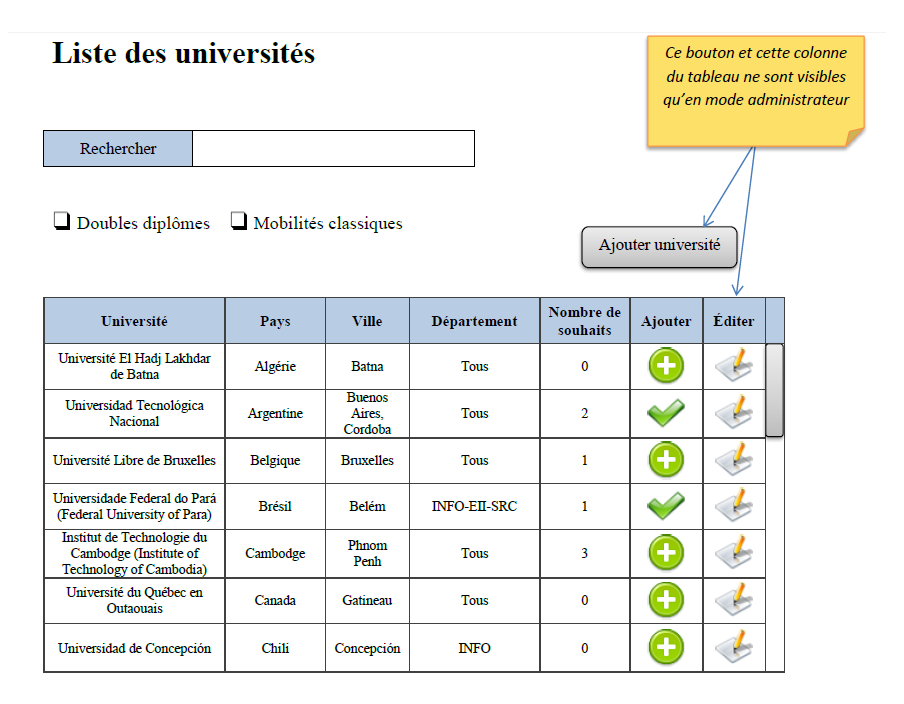
\includegraphics[scale=0.7]{Universites/listeUnivs.png}


Une page de notre application servira à renseigner la liste des destinations accessibles aux étudiants.
Les universités seront regroupées dans un tableau, pour lequel chaque ligne présentera les informations suivantes :
 \begin{itemize}
 	\item le nom de l'université partenaire
 	\item le pays dans laquelle elle se trouve
 	\item les départements pour lesquels cette destination est disponible
 	\item s'il s'agit d'un double diplôme
 	\item le nombres d'étudiants ayant fait ce vœux du/des département(s) sélectionné(s)
 	\item un bouton, à disposition des étudiants, pour ajouter cette destination à leur liste de vœux

 \end{itemize}
 
  Pour faciliter son parcours, une barre de recherche fonctionnant par mot-clef sera disponible au dessus du tableau. Un utilisateur pourra aussi sélectionner des filtres en haut du tableau. Il pourra filtrer par département ou pays en sélectionnant un choix parmi un menu déroulant. L'utilisateur pourra aussi cocher les cases "Doubles diplômes" ou "Mobilité classiques". Pour accéder à la fiche d'une université, il suffira de cliquer sur la ligne correspondante (sauf pour le bouton "Ajouter"). Si une destination figure déjà parmi les vœux de l'étudiant, la case "Ajouter" le figurera avec une icône différente.
  
  Il y a dissociation entre les doubles diplômes et les mobilités classiques. Si une destination propose les deux, un étudiant pourrait demander deux fois la destination pour chaque type de mobilité. Ce choix se fera dans une fenêtre apparaissant en cliquant sur "Ajout". 
 
 Les admins auront aussi à disposition des boutons pour éditer chaque destination, dont un bouton pour définir si le partenariat est actif ou non. Un partenariat inactif ne sera pas visible pour les étudiants.
 L'édition d'une entrée du tableau les reconduira vers la fiche où se trouvent toutes les informations sur la destination.
 Les admins pourront aussi supprimer une université du tableau s'ils le souhaitent.
 
 Les admins auront aussi moyen d'ajouter des universités au tableau via un bouton. Ils devront alors remplir une fiche descriptive de la nouvelle destination. L'université sera ajoutée au tableau une fois la fiche validée. De plus, un bouton leur permettra de télécharger (upload et download) la liste des universités au format CSV.
 
